\subsection{Segmentation}
In our data set there were 181 slices each containing and image with the dimensions 256x256.  For each slice the segmentation described in the segmentation section of the report was performed to identify each of the known tissues within our dataset.  Figure \ref{fig:resultsHistogram} shows an example the histogram distribution along with their corresponding MRI. Note the distinct peaks of the histogram which corresponds the the distinct known tissues of the brain.\\ 

\begin{figure}[H]
  \centering
  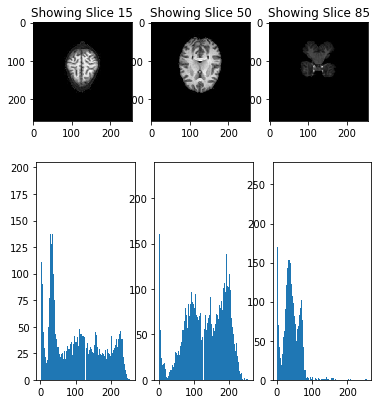
\includegraphics[width=\linewidth]{img/resultsHistogram.png}
  \caption{Brain slices of MRI with their corresponding histogram distribution.}
  \label{fig:resultsHistogram}
\end{figure}

Results of the manual seed region growing techniques and morphological filters can be seen in figure \ref{fig:resultsSegmentation}.

\begin{figure}[H]
  \centering
  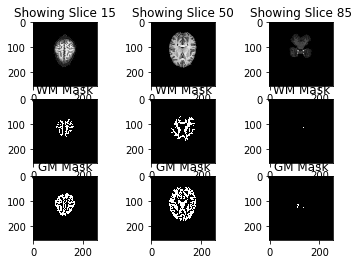
\includegraphics[width=\linewidth]{img/resultsSegmentation.png}
  \caption{\textbf{Top Row:} Original MRI. \textbf{Middle Row:}White matter mask. \textbf{Bottom Row:}Gray matter mask.}
  \label{fig:resultsSegmentation}
\end{figure}

We applied this technique not only for the regular brain but also for a brain which contains a tumor.  The following set of figures shows examples slices as well as their resultant class labels and individual mask layers.

\begin{figure}[H]
  \centering
  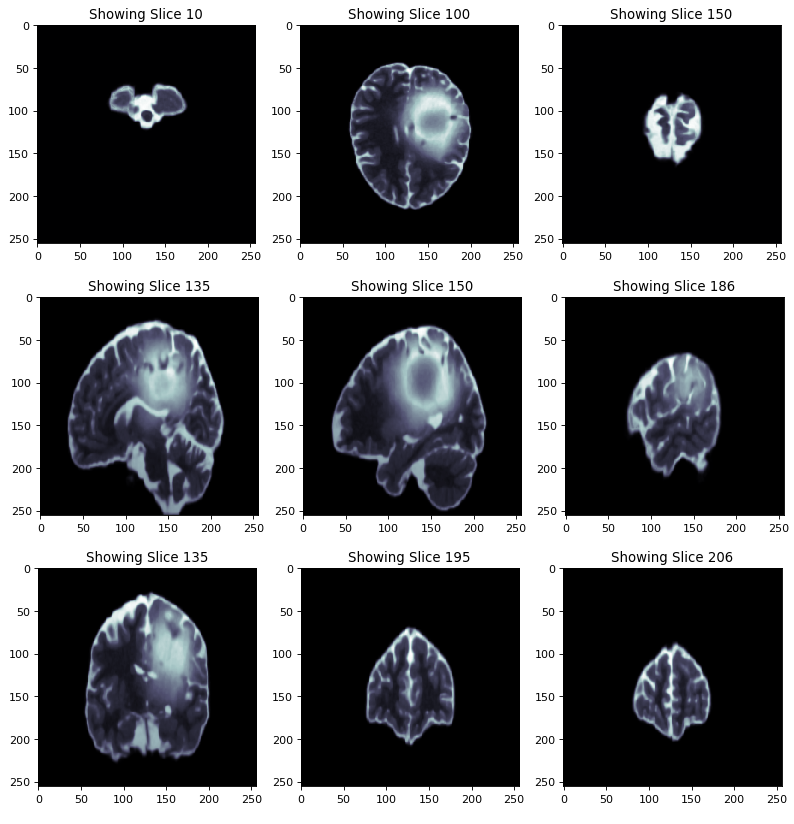
\includegraphics[width=\linewidth]{img/originalMRI.png}
  \caption{Original MRI slices in different views.  From top to bottom they are sliced in the axial, sagittal and coronal planes.}
  \label{fig:originalMRI}
\end{figure}

Note: the following images might look distorted and they are, and the reason is that because we have limited number of slices interpolation must be done to resize the image to its original width and height. Note the deformation of the coronal and sagittal views because of the limited depth data. Regardless I think we can use these views to narrow down the slices of interest.

\begin{figure}[H]
  \centering
  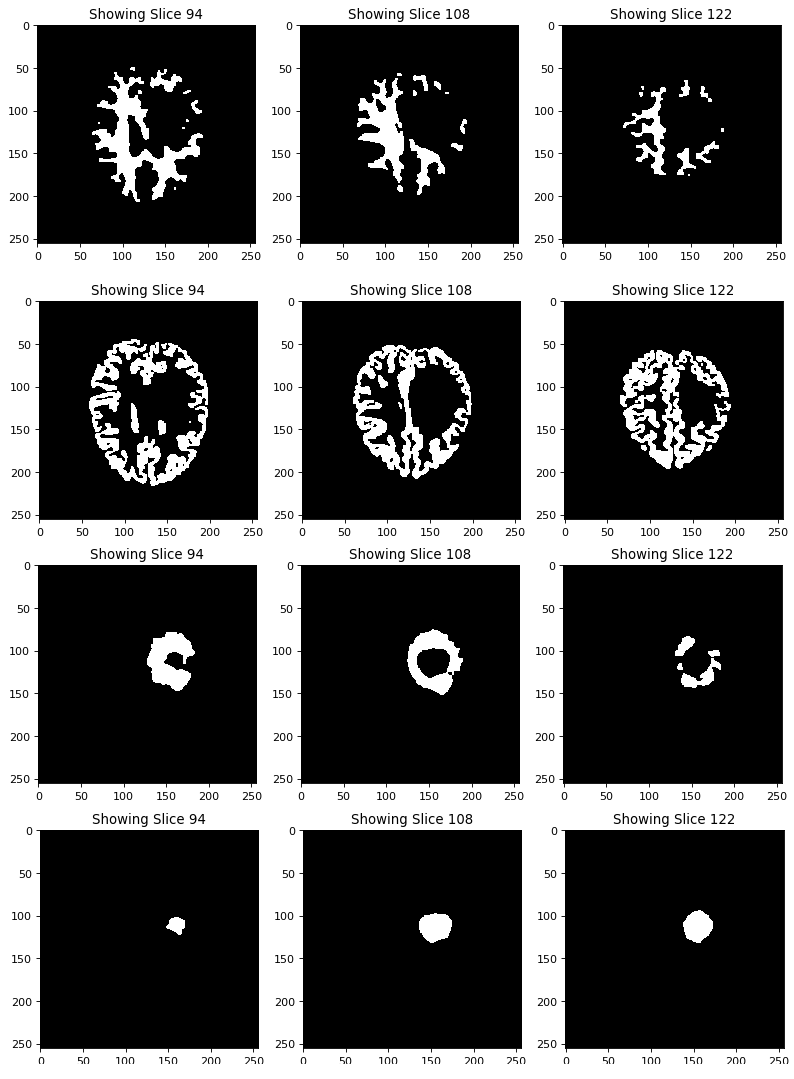
\includegraphics[width=\linewidth]{img/resultantMasks.png}
  \caption{Generated masks for each of the known tissue classes in our dataset.  From top to bottom they are: gray matter, white matter, abnormal tissue, and tumor.}
  \label{fig:resultantMasks}
\end{figure}

Even though we applied morphological filters we can still see some noise within the images, specifically the speckle effects in the gray matter and some holes in the white matter masks.  We can manually remove this again we can't because we can't modify data.

\begin{figure}[H]
  \centering
  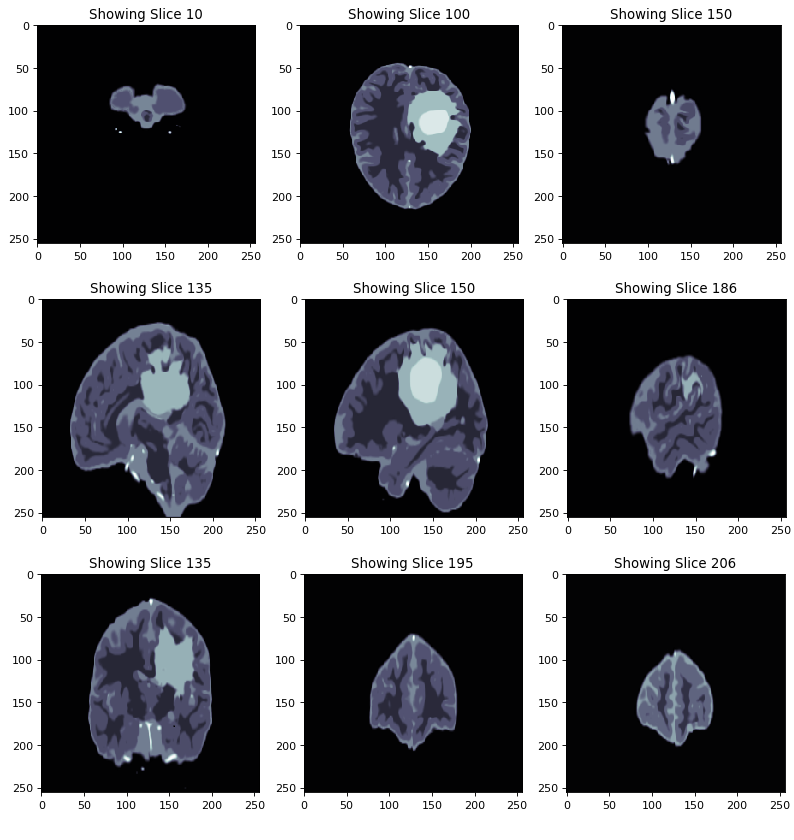
\includegraphics[width=\linewidth]{img/labeledMasks.png}
  \caption{Various slices and views of each of the coloured masks as found in the histogram.}
  \label{fig:labeledMasks}
\end{figure}

Each unique colour corresponds to a unique known tissue type.  By looking at various views you can get a picture as to where to tumor maybe located.  To create contrast between each distinct region we proposed the following colouring scheme.

\begin{figure}[H]
  \centering
  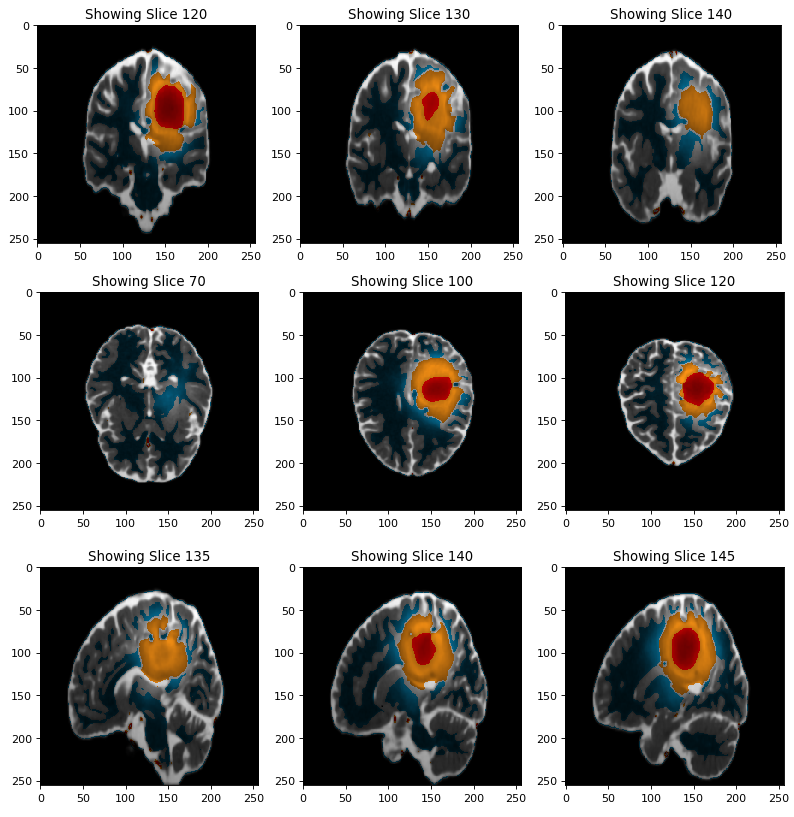
\includegraphics[width=\linewidth]{img/colourCodedRegions.png}
  \caption{}
  \label{fig:colourCodedRegions}
\end{figure}

\begin{table}[h]
\centering
\begin{tabular}{|r|l|l|l|}
\hline
Tissue & R & \multicolumn{1}{c|}{G} & B \\ \hline
White & 7 & \multicolumn{1}{c|}{150} & 204 \\ \hline
Gray & 204 & 204 & 204 \\ \hline
Abnormal Tissue & 203 & 119 & 17 \\ \hline
Tumor & 203 & 2 & 2 \\ \hline
\end{tabular}
\caption{RGB values of each of the tissue types.}
\label{table:RGBValues}
\end{table}

Notice that for each of the tissue types they can be clearly distinguish from each other. 

All codes that generated this section can be found in Appendix \ref{sec:appendixPythonMain}.